% TEMPLATE for Usenix papers, specifically to meet requirements of
%  USENIX '05
% originally a template for producing IEEE-format articles using LaTeX.
%   written by Matthew Ward, CS Department, Worcester Polytechnic Institute.
% adapted by David Beazley for his excellent SWIG paper in Proceedings,
%   Tcl 96
% turned into a smartass generic template by De Clarke, with thanks to
%   both the above pioneers
% use at your own risk.  Complaints to /dev/null.
% make it two column with no page numbering, default is 10 point

% Munged by Fred Douglis <douglis@research.att.com> 10/97 to separate
% the .sty file from the LaTeX source template, so that people can
% more easily include the .sty file into an existing document.  Also
% changed to more closely follow the style guidelines as represented
% by the Word sample file.

% Note that since 2010, USENIX does not require endnotes. If you want
% foot of page notes, don't include the endnotes package in the
% usepackage command, below.

% This version uses the latex2e styles, not the very ancient 2.09 stuff.
\documentclass[letterpaper,twocolumn,10pt]{article}
\usepackage{usenix,epsfig}
\usepackage{setup}

\newif\ifpublic
\publictrue

\newif\iffull
\fulltrue

\newtheorem{theorem}{Theorem}[section]
\newtheorem{lemma}[theorem]{Lemma}
\newtheorem{proposition}[theorem]{Proposition}
\newtheorem{corollary}[theorem]{Corollary}

\newcommand\invisiblesection[1]{%
  \refstepcounter{section}
\sectionmark{#1}}

\newenvironment{proof}[1][Proof]{\begin{trivlist}
\item[\hskip \labelsep {\bfseries #1}]}{\end{trivlist}}
  \newenvironment{definition}[1][Definition]{\begin{trivlist}
\item[\hskip \labelsep {\bfseries #1}]}{\end{trivlist}}
  \newenvironment{example}[1][Example]{\begin{trivlist}
\item[\hskip \labelsep {\bfseries #1}]}{\end{trivlist}}
  \newenvironment{remark}[1][Remark]{\begin{trivlist}
\item[\hskip \labelsep {\bfseries #1}]}{\end{trivlist}}

  \newcommand{\qed}{\nobreak \ifvmode \relax \else
    \ifdim\lastskip<1.5em \hskip-\lastskip
    \hskip1.5em plus0em minus0.5em \fi \nobreak
  \vrule height0.75em width0.5em depth0.25em\fi}


% \DeclareMathOperator*{\argmin}{arg\,min}
% \DeclareMathOperator*{\Vol}{Vol}
% \DeclareMathOperator*{\Supp}{Supp}
% \newcommand{\cR}{\ensuremath{\mathcal R}}
% \newcommand{\cS}{\ensuremath{\mathcal S}}
%
% \newcommand{\CVPDf}{\ensuremath{\algo{CVP}_{\tilde{D}_4}}}
% \newcommand{\CVPDfZf}{\ensuremath{\algo{CVP}_{D_4/\ZZ^4}}}
% \newcommand{\LDEncode}{\algo{Encode}}
% \newcommand{\LDDecode}{\algo{Decode}}



\usepackage{soul}\let\strikethrough\st\let\st\undefined

% \newcommand{\T}{L}

\newcommand{\Z}{\ensuremath{\mathbb{Z}}}
\newcommand{\K}{\ensuremath{\mathbb{K}}}
\newcommand{\ZZ}{\ensuremath{\mathbb{Z}}}
\newcommand{\corr}{\,\hat{=}\,}
\newcommand{\B}{\ensuremath{\mathbb{B}}}
\newcommand{\E}{\ensuremath{\mathbb{E}}}
\newcommand{\Oinf}{\ensuremath{\mathcal{O}}}
\newcommand{\F}[1]{\ensuremath{\mathbb{F}_{#1}}}

% \newcommand{\RR}{\ensuremath{\mathbb{R}}}
\newcommand{\N}{\ensuremath{\mathbb{N}}}

\newcommand{\mbf}{\ensuremath{\mathbf}}
% \newcommand{\rando}{\ensuremath{\xleftarrow{\$}}}
% \newcommand{\la}{\ensuremath{\leftarrow}}

% \newcommand{\MD}{\ensuremath{\mathcal{D}}\xspace}
% \newcommand{\MS}{\ensuremath{\mathcal{D}}\xspace}
% \newcommand{\MA}{\ensuremath{\mathcal{A}}\xspace}
% \newcommand{\MB}{\ensuremath{\mathcal{B}}\xspace}
% \newcommand{\MP}{\ensuremath{\mathcal{P}}\xspace}
% \newcommand{\tA}{\ensuremath{t_{\mathcal{A}}}}
% \newcommand{\eA}{\ensuremath{\varepsilon_{\mathcal{A}}}}
% \newcommand{\tS}{\ensuremath{t_{\mathcal{D}}}}
% \newcommand{\eS}{\ensuremath{\varepsilon_{\mathcal{D}}}}

% \newcommand{\vX}{\mathcal X}
% \newcommand{\vY}{\mathcal Y}


% \newcommand{\MR}{\ensuremath{\mathcal{R}}\xspace}
% \newcommand{\tR}{\ensuremath{t_{\mathcal{R}}}}
% \newcommand{\eR}{\ensuremath{\varepsilon_{\mathcal{R}}}}
%
% \newcommand{\tD}{\ensuremath{t_{\mathcal{D}}}}
% \newcommand{\eD}{\ensuremath{\varepsilon_{\mathcal{D}}}}
% \newcommand{\sis}{\textsf{SIS}\xspace}
% \newcommand{\isis}{\textsf{ISIS}\xspace}
% \newcommand{\lwe}{\textsf{LWE}\xspace}
% \newcommand{\dlwe}{\textsf{LWE}\xspace}
% \newcommand{\rdlwe}{\textsf{R-LWE}\xspace}
%
% \newcommand{\ee}{\ensuremath{\varepsilon}}
%
% \newcommand{\sS}{\ensuremath{\sigma}}
% \newcommand{\sE}{\ensuremath{\sigma}}
% \newcommand{\DS}{\ensuremath{D_{\sS}}}
% \newcommand{\DE}{\ensuremath{D_{\sE}}}
% %\newcommand{\Dy}{\ensuremath{D_y}}
% \newcommand{\Dy}{\ensuremath{[-B, B]}}
% \newcommand{\Dysc}{\ensuremath{D_{y,\mat{Sc}}}}
% \newcommand{\Dz}{\ensuremath{D_z}}
% \newcommand{\bit}{\ensuremath{\{0,1\}}}
% \newcommand{\eqdef}{\stackrel{\mathrm{def}}=}
% \newcommand{\rand}{\getsr}

% \newcommand{\rounddq}[1]{\ensuremath{\lfloor #1 \rceil_{d,q}}}
% \newcommand{\roundd}[1]{\ensuremath{\lfloor #1 \rceil_d}}
% \newcommand{\norm}[1]{\ensuremath{||#1||}}

% \newcommand{\KeyGen}{\keygen}
% \newcommand{\Sign}{\sign}
% \newcommand{\Verify}{\verify}
% \newcommand{\keygen}{\ensuremath{\mathsf{KeyGen}}}
% \newcommand{\sign}{\ensuremath{\mathsf{Sign}}}
% \newcommand{\verify}{\ensuremath{\mathsf{Verify}}}
% \newcommand{\start}{\underline{\ensuremath{\mathsf{Start}}}\xspace}
% \newcommand{\randO}{\ensuremath{\underline{\mathsf{Rand}}^{O_c}}\xspace}
% \newcommand{\signO}{\ensuremath{\underline{\mathsf{Sign}}^{O_c}}\xspace}
% \newcommand{\finishO}{\ensuremath{\underline{\mathsf{Finish}}^{O_c}}}
% \newcommand{\instance}{\underline{\ensuremath{\mathsf{Instance}}}}
% \newcommand{\Sample}{\ensuremath{\mathsf{Sample}}}

% \newcommand{\keygenQ}{\ensuremath{\mathsf{KeyGen}}}
% \newcommand{\signQ}{\ensuremath{\mathsf{Sign}}}
% \newcommand{\verifyQ}{\ensuremath{\mathsf{Verify}}}
% \newcommand{\CHgen}{\ensuremath{\mathsf{ChGen}}}

% \newcommand{\inputtext}{\textsf{INPUT:}\;}
% \newcommand{\outputtext}{\textsf{OUTPUT:}\;}
% \newcommand{\iftext}{\mathbf{if\;}}
% \newcommand{\elsetext}{\mathbf{else\;}}
% \newcommand{\then}{\mathbf{then\;}}
% \newcommand{\return}{\mathbf{return\;}}

% \newcommand{\mat}[1]{\mathbf{#1}}
% \renewcommand{\vec}[1]{\mathbf{#1}}
% \newcommand{\modq}{\ensuremath{\; (\bmod \; q)}}
%\newcommand{\modq}{\ensuremath{\; (q)}}
% \newcommand{\ip}[2]{\ensuremath{\langle {#1},{#2}\rangle}}

% \newcommand{\adv}{\ensuremath{\mathcal{A}}}
% \newcommand{\secpar}{\ensuremath{\lambda}}

% \newcommand{\sk}{\ensuremath{\mathsf{sk}}\xspace}
% \newcommand{\pk}{\ensuremath{\mathsf{vk}}\xspace}
% \newcommand{\sst}{\ensuremath{\mathsf{st}}\xspace}

% \newcommand{\CH}{\ensuremath{\mathcal{CH}}}
% \newcommand{\ch}{\ensuremath{\mathsf{CH}}}
% \newcommand{\Mek}{\ensuremath{\mathsf{M_{ek}}}}
% \newcommand{\Yek}{\ensuremath{\mathsf{Y_{ek}}}}
% \newcommand{\Rek}{\ensuremath{\mathsf{R_{ek}}}}
% \newcommand{\ek}{\ensuremath{\mathsf{ek}}}
% \newcommand{\td}{\ensuremath{\mathsf{td}}}
% \newcommand{\Gen}{\ensuremath{\mathsf{Gen}}}

% \newcommand{\negl}{\ensuremath{\mathsf{negl}}}


% \newcommand{\R}{\mathcal{R}}
% \newcommand{\Rp}{\mathcal{R}_p}
% \newcommand{\Rq}{\mathcal{R}_q}
% \newcommand{\Rqk}[1]{\mathcal{R}_{q,#1}}

% \def\getsr{\stackrel{{\scriptscriptstyle \$}}{\leftarrow}}
% \def\gets{{\leftarrow}}


% \newcommand{\Uniform}{\mathcal{U}}
% \newcommand{\UniRk}[1]{\Rqk{#1}}
% \newcommand{\UniRq}{\Rq}


\newcommand{\zeropo}{{\bf 0}}
\newcommand{\Apo}{{\bf A\xspace}}
\newcommand{\Bpo}{{\bf B\xspace}}
\newcommand{\Ipo}{{\bf I\xspace}}
\newcommand{\apo}{{\bf a\xspace}}
\newcommand{\bpo}{{\bf b\xspace}}
\newcommand{\cpo}{{\bf c\xspace}}
\newcommand{\Cpo}{{\bf C\xspace}}
\newcommand{\dpo}{{\bf d\xspace}}
\newcommand{\epo}{{\bf e\xspace}}
\newcommand{\ppo}{{\bf p\xspace}}
\newcommand{\fpo}{{\bf f\xspace}}
\newcommand{\gpo}{{\bf g\xspace}}
\newcommand{\Gpo}{{\bf G\xspace}}
\newcommand{\hpo}{{\bf h\xspace}}
\newcommand{\kpo}{{\bf k\xspace}}
\newcommand{\Kpo}{{\bf K\xspace}}
\newcommand{\lpo}{{\bf l\xspace}}
\newcommand{\Lpo}{{\bf L\xspace}}
\newcommand{\mpo}{{\bf m\xspace}}
\newcommand{\rpo}{{\bf r\xspace}}
\newcommand{\spo}{{\bf s\xspace}}
\newcommand{\tpo}{{\bf t\xspace}}
\newcommand{\upo}{{\bf u\xspace}}
\newcommand{\Upo}{{\bf U\xspace}}
\newcommand{\vpo}{{\bf v\xspace}}
\newcommand{\wpo}{{\bf w\xspace}}
\newcommand{\xpo}{{\bf x\xspace}}
\newcommand{\ypo}{{\bf y\xspace}}
\newcommand{\zpo}{{\bf z\xspace}}
\newcommand{\Zpo}{{\bf Z\xspace}}

\newcommand{\Spo}{{\bf S}}
\newcommand{\Ypo}{{\bf Y}}

% \newcommand{\algo}[1]{\textsf{#1}}

% \newcommand{\PeikertDBL}{\algo{dbl}}
% \newcommand{\PeikertREC}{\algo{rec}}


% \newcommand{\PowMul}{{\text{\sf PowMul}}}
% \newcommand{\PowMulPsi}{{\text{\sf PowMul}_{\psi}}}
\newcommand{\ie}{{\textit{i.e.}}\;}
\newcommand{\eg}{{\textit{e.g.}}\;}
\newcommand{\p}{\ensuremath{2^{255}-19}}
\newcommand{\Zfield}{\ensuremath{\mathbb{Z}_{\p}}}
\newcommand{\Ffield}{\ensuremath{\mathbb{F}_{\p}}}


\begin{document}

%don't want date printed
\date{}

%make title bold and 14 pt font (Latex default is non-bold, 16 pt)
\title{\Large \bf Proving the complete correctness of TweetNaCl's Curve25519 implementation.%
\thanks{
Date: somewhen in 2018.}
}

%for single author (just remove % characters)
\ifpublic
\author{
{\rm Peter Schwabe}\\
  Radboud University, The Netherlands\\
%\~\\
\and
{\rm Beno\^it Viguier}\\
  Radboud University, The Netherlands\\
%\~\\
\and
{\rm Timmy Weerwag}\\
  Radboud University, The Netherlands\\
%\~\\
\and
{\rm Freek Wiedijk}\\
  Radboud University, The Netherlands\\
}
\fi

\maketitle

%\thispagestyle{empty}

\subsection*{Abstract}
By using the Coq formal proof assistant with the VST library, we prove the
soundness and correctness of TweetNaCl's Curve25519 implementation.

\section{Introduction}

Implementing cryptographic primitives without any bugs is hard.
While tests provides a code coverage and are used in the limits,
they still don't cover 100\% of the possible input values.

In order to get formal guaranties a software meets its specifications,
two methodologies exist. The first one is by synthesizing a formal specification and
generating machine code by refinment. This approach is being used in the
B-method\cite{Abrial:1996:BAP:236705}, F* \cite{DBLP:journals/corr/BhargavanDFHPRR17} with Kremlin, or in Coq \cite{CpdtJFR}.
This gives you a software correct by construction. However it cannot be applied
to an existing piece of software. In such case we need to write the specifications
and then verify the correctness of the implementation.

Verifying an existing cryptographic library, we use the second approach.
Our method can be seen as a static analysis over the input values coupled
with the formal proof that the code of the algorithm matches its specification.
Similar approaches have been used to prove the correctness of OpenSSL HMAC
\cite{Beringer2015VerifiedCA} and SHA-256 \cite{Appel2015VerificationOA}.

TweetNaCl\cite{BGJ+15} is a compact reimplementation of the
NaCl\cite{BLS12} library. It does not aim for high speed
application and has been optimized for source code compactness.
It maintains some degree of readability in order to be easily auditable.

This library makes use of Curve25519\cite{Ber06}, a function over a \F{p}-restricted
$x$-coordinate computing a scalar multiplication on $E(\F{p^2})$, where $p$ is
the prime number \p and $E$ is the elliptic curve $y^2 = x^3 + 486662 x^2 + x$.

Coq is a formal system that allows to machine-check our proofs.
A famous example of its use is the proof of the Four Color Theorem.
The Compcert\cite{Leroy-backend} compiler and the Verifiable Software Toolchain
(VST)\cite{2012-Appel} are build on top of it.

Our approach is as follow, we use the \textit{clightgen} tool from Compcert to
generate the \textit{semantic version} (Clight\cite{Blazy-Leroy-Clight-09}) of
the TweetNaCl C code.
Using the Separation logic\cite{1969-Hoare,Reynolds02separationlogic}
with with the Verifiable Software Toolchain we show that the semantics of the
program satisfies a functionnal specification in Coq.
We extend the work of Bartzia and Strub \cite{DBLP:conf/itp/BartziaS14} to
support Montgomery curves.
With this formalization, we prove the correctness of a generic Montgomery ladder
and show that our specification can be seen as an instance of it.

% Five years ago:
% \url{https://www.imperialviolet.org/2014/09/11/moveprovers.html}
% \url{https://www.imperialviolet.org/2014/09/07/provers.html}

% \section{Related Works}
%
% \begin{itemize}
%   \item HACL*
%   \item Proving SHA-256 and HMAC
%   \item \url{http://www.iis.sinica.edu.tw/~bywang/papers/ccs17.pdf}
%   \item \url{http://www.iis.sinica.edu.tw/~bywang/papers/ccs14.pdf}
%   \item \url{https://cryptojedi.org/crypto/#gfverif}
%   \item \url{https://cryptojedi.org/crypto/#verify25519}
%   \item Fiat Crypto : synthesis
% \end{itemize}
%
% Add comparison with Fiat-crypto

\section{Curve25519 implementation}

In order to prove the correctness of \texttt{crypto\_scalarmult},
 we also need to do the same with all the functions subsequently called:
\texttt{unpack25519}; \texttt{A}; \texttt{Z}; \texttt{M}; \texttt{S};
\texttt{car25519}; \texttt{inv25519}; \texttt{set25519}; \texttt{sel25519};
\texttt{pack25519}.

\subsection{Implementation} \label{sec:impl}

Curve25519 is defined over $\mathbb{Z}_{2^{255}-19}$. Number in that field can
be represented by a 256-bits number. Each of them represented in base $2^{16}$.
they are cut into 16 limbs of at least 16 bits placed into 64-bits signed
container.

\begin{lstlisting}[language=Ctweetnacl]
typedef long long i64;
typedef i64 gf[16];
\end{lstlisting}
This does not guaranty a unique representation of each number. i.e.\\
$\exists x,y \in$ \TNaCle{gf} such that
\vspace{-0.25cm}
  $$x \neq y\ \ \land\ \ x \equiv y \pmod{2^{255}-19}$$

On the other hand it allows simple definitions of addition (\texttt{A}),
substraction (\texttt{Z}) and a (school-book) multiplication (\texttt{M}).
\begin{lstlisting}[language=Ctweetnacl]
sv A(gf o,const gf a,const gf b) {
  int i;
  FOR(i,16) o[i]=a[i]+b[i];
}

sv Z(gf o,const gf a,const gf b) {
  int i;
  FOR(i,16) o[i]=a[i]-b[i];
}

sv M(gf o,const gf a,const gf b) {
  i64 i,j,t[31];
  FOR(i,31) t[i]=0;
  FOR(i,16) FOR(j,16) t[i+j]+=a[i]*b[j];
  FOR(i,15) t[i]+=38*t[i+16];
  FOR(i,16) o[i]=t[i];
  car25519(o);
  car25519(o);
}
\end{lstlisting}

To avoid overflows, carries are propagated by the \texttt{car25519} function.
\begin{lstlisting}[language=Ctweetnacl]
sv car25519(gf o) {
  int i;
  i64 c;
  FOR(i,15) {
    o[i]+=(1LL<<16);
    c=o[i]>>16;
    o[(i+1)*(i<15)]+=c-1+37*(c-1)*(i==15);
    o[i]-=c<<16;
  }
}
\end{lstlisting}

At the end of the Mongomery ladder, we have to compute an inverse.
This is done using the Fermat's little theorem by the exponentiation to
$2^{255}-21$ with the Square-and-multiply algorithm and taking
advantage of the shape of the number.
\begin{lstlisting}[language=Ctweetnacl]
sv inv25519(gf o,const gf a)
{
  gf c;
  int i;
  set25519(c,a);
  for(i=253;i>=0;i--) {
    S(c,c);
    if(i!=2&&i!=4) M(c,c,a);
  }
  FOR(i,16) o[i]=c[i];
}
\end{lstlisting}

The last step of the crypto\_scalarmult is the packing of the limbs, it returns
an array of bytes and guarantees a unique representation in $\mathbb{Z}_{2^{255}-19}$.
\begin{lstlisting}[language=Ctweetnacl]
sv pack25519(u8 *o,const gf n)
{
  int i,j;
  i64 b;
  gf t,m={0};
  set25519(t,n);
  car25519(t);
  car25519(t);
  car25519(t);
  FOR(j,2) {
    m[0]=t[0]- 0xffed;
    for(i=1;i<15;i++) {
      m[i]=t[i]-0xffff-((m[i-1]>>16)&1);
      m[i-1]&=0xffff;
    }
    m[15]=t[15]-0x7fff-((m[14]>>16)&1);
    m[14]&=0xffff;
    b=1-((m[15]>>16)&1);
    sel25519(t,m,b);
  }
  FOR(i,16) {
    o[2*i]=t[i]&0xff;
    o[2*i+1]=t[i]>>8;
  }
}
\end{lstlisting}

The full Montgomery ladder is defined as follow:
\begin{lstlisting}[language=Ctweetnacl]
int crypto_scalarmult(u8 *q,
                      const u8 *n,
                      const u8 *p)
{
  u8 z[32];
  i64 r;
  int i;
  gf x,a,b,c,d,e,f;
  FOR(i,31) z[i]=n[i];
  z[31]=(n[31]&127)|64;
  z[0]&=248;
  unpack25519(x,p);
  FOR(i,16) {
    b[i]=x[i];
    d[i]=a[i]=c[i]=0;
  }
  a[0]=d[0]=1;
  for(i=254;i>=0;--i) {
    r=(z[i>>3]>>(i&7))&1;
    sel25519(a,b,r);
    sel25519(c,d,r);
    A(e,a,c);
    Z(a,a,c);
    A(c,b,d);
    Z(b,b,d);
    S(d,e);
    S(f,a);
    M(a,c,a);
    M(c,b,e);
    A(e,a,c);
    Z(a,a,c);
    S(b,a);
    Z(c,d,f);
    M(a,c,_121665);
    A(a,a,d);
    M(c,c,a);
    M(a,d,f);
    M(d,b,x);
    S(b,e);
    sel25519(a,b,r);
    sel25519(c,d,r);
  }
  inv25519(c,c);
  M(a,a,c);
  pack25519(q,a);
  return 0;
}
\end{lstlisting}

\subsection{What need to be proven?}

We prove that the implementation of Curve25519 is \textbf{sound} \ie

\begin{itemize}
\item absence of access out-of-bounds of arrays.
\item absence of overflows/underflow on the arithmetic.
\end{itemize}

We also prove that TweetNaCl's code is \textbf{correct}:

\begin{itemize}
\item Curve25519 is correctly implemented (we get what we expect).
\item Operations on \texttt{gf} (\texttt{A}, \texttt{Z}, \texttt{M}, \texttt{S})
are equivalent to operations ($+,-,\times,x^2$) in $\mathbb{Z}_{2^{255}-19}$
\end{itemize}

% \subsection{Meet-in-the-middle Approach}

In order to prove the soundness and correctness of \texttt{crypto\_scalarmult},
we defined multiples levels of specifications.
A high level specification (over a generic field $\mathbb{F}$) looking only at
the structure of the Montgomery ladder provided us with the correcntess.
A low level specification close to the \texttt{C} code (over lists of $\mathbb{Z}$)
gave us the soundness assurance.
We defined a third specification over $\mathbb{Z}_{2^{255}-19}$ (mid level) and
we proved to be an instance of the high level one.
We also proved its equivalence with the low level one.
As such we proved all specifications to equivalent (Fig.\ref{tk:ProofStructure}).
This garantees us the correctness of the
implementation.

\begin{figure}[h]
  \begin{tikzpicture}[textstyle/.style={black, anchor= south west, align=center}]

    \filldraw[draw=orange!10!doc@lstbackground, fill=doc@lstbackground, thick] (0.25,0.5) rectangle (4.5,5.5);
    % node[textstyle, anchor=west, draw=yellow, fill=yellow!20, thick, minimum width=5.5cm,minimum height=5cm] {};

    \draw (4.5,5.5)  node[anchor=north east, inner sep=0pt] (russell) {
\includegraphics[width=.03\textwidth]{img/coq_logo.png}};

    \draw (0.5,-1) node [textstyle, anchor=west, draw=black, thick, minimum width=3cm,minimum height=0.5cm] (longlong) {\texttt{long long[16]}};
    \draw (0,-1) node [anchor=east] (longlongdef) {\texttt{C} code};
    \draw (2.25,-0.1) node [anchor=west] (app) {\texttt{clightgen}};


    \draw (0.5,1) node [textstyle, anchor=west, draw=black, thick, minimum width=3cm,minimum height=0.5cm] (clight) {\texttt{tptr tlong}};
    \draw (0,1) node [anchor=east] (clightdef) {Clight};

    \draw [thick, ->] (longlong.north) -- (clight.south);

    \begin{scope}[yshift=1 cm,xshift=0 cm]

      \draw (0.5,2) node [textstyle, anchor=west, draw=black, thick, minimum width=3cm,minimum height=0.5cm] (ll) {\texttt{list} $\Z$};
      \draw (0,2) node [anchor=east] (shn) {Low Level};

      \draw [thick,double, <->, >=implies] (clight.north) -- (ll.south);
      \draw (2.25,1) node[anchor=west, inner sep=0pt] (chain) {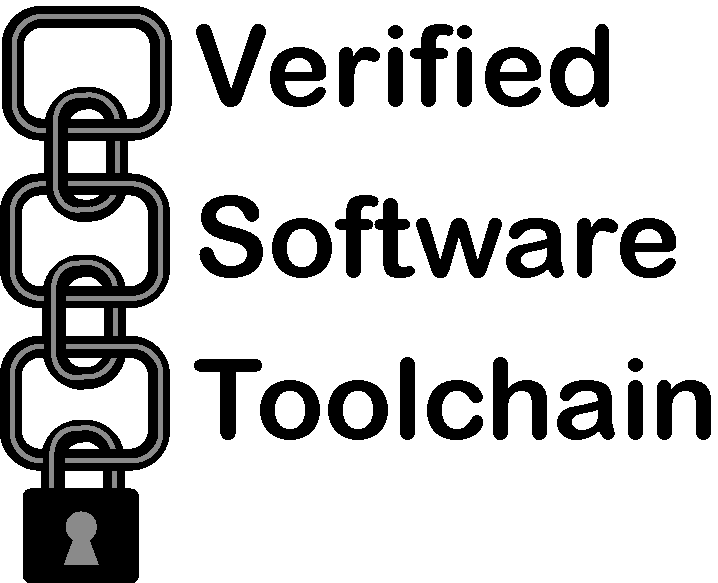
\includegraphics[width=.07\textwidth]{img/chain.png}};


      \draw (0.5,3) node [textstyle, anchor=west, draw=black, thick, minimum width=3cm,minimum height=0.5cm] (ml) {$\Zfield$};
      \draw (0,3) node [anchor=east] (shn) {Mid Level};

      \draw[thick,double, <->, >=implies] (ll.north) -- (ml.south);

      \draw (0.5,4) node [textstyle, anchor=west, draw=black, thick, minimum width=3cm,minimum height=0.5cm] (hl) {$\K$};
      \draw (0,4) node [anchor=east] (shn) {High Level};

      \draw[thick,double, <-, >=implies] (ml.north) -- (hl.south);
    \end{scope}
\end{tikzpicture}

  \caption{Structural construction of the proof}
  \label{tk:ProofStructure}
\end{figure}

\subsection{Correctness specification}

% The soundness is implied by the proof of the following specification.
We show the soundness of TweetNaCl by proving the {\red{equivalence}} of the following
specification. This defines the equivalence between the Clight representation
and a Coq definition of the ladder.

\begin{lstlisting}[language=CoqVST]
Definition crypto_scalarmult_spec :=
DECLARE _crypto_scalarmult_curve25519_tweet
WITH
  v_q: val, v_n: val, v_p: val, c121665:val,
  sh : share,
  q : list val, n : list Z, p : list Z
(*------------------------------------------*)
PRE [ _q OF (tptr tuchar),
     _n OF (tptr tuchar),
     _p OF (tptr tuchar) ]
PROP (writable_share sh;
      Forall (fun x => 0 <= x < 2^8) p;
      Forall (fun x => 0 <= x < 2^8) n;
      Zlength q = 32; Zlength n = 32;
      Zlength p = 32)
LOCAL(temp _q v_q; temp _n v_n; temp _p v_p;
      gvar __121665 c121665)
SEP  (sh [{ v_q }] <<(uch32)-- q;
      sh [{ v_n }] <<(uch32)-- mVI n;
      sh [{ v_p }] <<(uch32)-- mVI p;
      Ews [{ c121665 }] <<(lg16)-- mVI64 c_121665)
(*------------------------------------------*)
POST [ tint ]
PROP (Forall (fun x => 0 <= x < 2^8) (CSM n p);
      Zlength (CSM n p) = 32)
LOCAL(temp ret_temp (Vint Int.zero))
SEP  (sh [{ v_q }] <<(uch32)-- mVI (CSM n p);
      sh [{ v_n }] <<(uch32)-- mVI n;
      sh [{ v_p }] <<(uch32)-- mVI p;
      Ews [{ c121665 }] <<(lg16)-- mVI64 c_121665
\end{lstlisting}

In this specification we state as preconditions:
\begin{itemize}
  \item[] \VSTe{PRE}: \VSTe{_p OF (tptr tuchar)}\\
  The function \texttt{crypto\_scalarmult} takes as input three pointers to
  arrays of unsigned bytes (\VSTe{tptr tuchar}) \VSTe{_p}, \VSTe{_q} and \VSTe{_n}.
  \item[] \VSTe{LOCAL}: \VSTe{temp _p v_p}\\
  Each pointer represent an address \VSTe{v_p},
  \VSTe{v_q} and \VSTe{v_n}.
  \item[] \VSTe{SEP}: \VSTe{sh [{ v_p $\!\!\}\!\!]\!\!\!$ <<(uch32)-- mVI p}\\
  In the memory share \texttt{sh}, the address \VSTe{v_p} points
  to a list of integer values \VSTe{mVI p}.
  \item[] \VSTe{PROP}: \VSTe{Forall (fun x => 0 <= x < 2^8) p}\\
  In order to consider all the possible inputs, we assumed each
  elements of the list \texttt{p} to be bounded by $0$ included and $2^8$
  excluded.
  \item[] \VSTe{PROP}: \VSTe{Zlength p = 32}\\
  We also assumed that the length of the list \texttt{p} is 32. This defines the
  complete representation of \TNaCle{u8[32]}.
\end{itemize}

As Post-condition we have:
\begin{itemize}
  \item[] \VSTe{POST}: \VSTe{tint}\\
  The function \texttt{crypto\_scalarmult} returns an integer.
  \item[] \VSTe{LOCAL}: \VSTe{temp ret_temp (Vint Int.zero)}\\
  The returned integer has value $0$.
  \item[] \VSTe{SEP}: \VSTe{sh [{ v_q $\!\!\}\!\!]\!\!\!$ <<(uch32)-- mVI (CSM n p)}\\
  In the memory share \texttt{sh}, the address \VSTe{v_q} points
  to a list of integer values \VSTe{mVI (CSM n p)}.
  \item[] \VSTe{PROP}: \VSTe{Forall (fun x => 0 <= x < 2^8) (CSM n p)}\\
  \VSTe{PROP}: \VSTe{Zlength (CSM n p) = 32}\\
  We show that the computation for \VSTe{CSM} fits in  \TNaCle{u8[32]}.
\end{itemize}

\texttt{THEOREM BETWEEN CSM and TIMMY REPR. EG:}
\begin{lstlisting}[language=CoqD]
Theorem CSM_eq :
  forall (n:list Z) (p:list Z),
  Zlength n = 16 ->
  Zlength p = 16 ->
  Forall (fun x => 0 <= x < 2^8) p ->
  Forall (fun x => 0 <= x < 2^8) n ->
  Z16.lst (CSM n p) = Z16.lst n $\times$ Z16.lst p.
\end{lstlisting}
We proved that \VSTe{crypto_scalarmult} (\VSTe{CSM} in Coq)
computes: $$Q.x \leftarrow N \times P.x$$

where \VSTe{p} represent the x-coordinate of $P$, \VSTe{n} represent the
scalar by which it is be multiplied $N$ (where the bits 1, 2, 5 248, 249, 250
are cleared and bit 6 is set).

% As a result of the excution of \VSTe{crypto_scalarmult}, the value \VSTe{0}
% is returned, \VSTe{p} and \VSTe{n} points to the same locations containing
% the same values \VSTe{pp} and \VSTe{nn}.
% The pointer \VSTe{q} points to the same location, but contain the x coordinate of $Q$.

\section{Mathematical Model}

In this section we first present the work of Bartzia and Strub \cite{DBLP:conf/itp/BartziaS14} (\ref{Weierstrass}).
We extend it to support Montgomery curves (\ref{montgomery}) with homogeneous coordinates (\ref{projective}) and prove the correctness of the ladder (\ref{ladder}).

We then prove the montgomery ladder computes
the x-coordinate of scalar multiplication over $\F{p^2}$
(Theorem 2.1 by Bernstein \cite{Ber06}) where $p$ is the prime $\p$.

\subsection{Formalization of Elliptic Curves}

We consider elliptic curves over a field $\K$. We assume that the
characteristic of $\K$ is neither 2 or 3.

\begin{definition}
Let a field $\K$, using an appropriate choice of coordinates, an elliptic curve $E$
is a plane cubic albreaic curve $E(x,y)$ defined by an equation of the form:
$$E : y^2 + a_1 xy + a_3 y = x^3 + a_2 x^2 + a_4 x + a_6$$
where the $a_i$'s are in \K\ and the curve has no singular point (\ie no cusps
or self-intersections). The set of points, written $E(\K)$, is formed by the
solutions $(x,y)$ of $E$ augmented by a distinguished point $\Oinf$ (called point at infinity):
$$E(\K) = \{(x,y) \in \K \times \K | E(x,y)\} \cup \{\Oinf\}$$
\end{definition}

\subsubsection{Weierstra{\ss} curves}
\label{Weierstrass}
This equation $E(x,y)$ can be reduced into its Weierstra{\ss} form.

\begin{definition}
Let $a \in \K$, and $b \in \K$ such that $$\Delta(a,b) = -16(4a^3 + 27b^2) \neq 0.$$ The \textit{elliptic curve} $E_{a,b}(\K)$ is the set of all points $(x,y) \in \K^2$ satisfying the equation:
$$y^2 = x^3 + ax + b,$$
along with an additional formal point $\Oinf$, ``at infinity''. Such curve does not present any singularity.
\end{definition}

In this setting, Bartzia and Strub defined the parametric type \texttt{ec} which
represent the points on a specific curve. It is parametrized by
a \texttt{K : ecuFieldType} -- the type of fields which characteristic is not 2 or 3 --
and \texttt{E : ecuType} -- a record that packs the curve parameters $a$ and $b$
along with the proof that $\Delta(a,b) \neq 0$.
\begin{lstlisting}[language=Coq]
Inductive point := EC_Inf | EC_In of K * K.
Notation "(| x, y |)" := (EC_In x y).
Notation "\infty" := (EC_Inf).

Record ecuType :=
  { A : K; B : K; _ : 4 * A^3 + 27 * B^2 != 0}.
Definition oncurve (p : point) :=
  if p is (| x, y |)
    then y^2 == x^3 + A * x + B
    else true.
Inductive ec : Type := EC p of oncurve p.
\end{lstlisting}

Points of an elliptic curve can be equiped with a structure of an abelian group.
\begin{itemize}
  \item The negation of a point $P = (x,y)$ by taking the symetric with respect to the x axis $-P = (x, -y)$.
  \item The addition of two points $P$ and $Q$ is defined by the negation of third intersection
  of the line passing by $P$ and $Q$ or tangent to $P$ if $P = Q$.
  \item $\Oinf$ is the neutral element under this law: if 3 points are colinear, their sum is equal to $\Oinf$.
\end{itemize}

This operaction can be defined in Coq as follow:
\begin{lstlisting}[language=Coq]
Definition neg (p : point) :=
  if p is (| x, y |) then (| x, -y |) else EC_Inf.

Definition add (p1 p2 : point) :=
  match p1, p2 with
    | \infty , _ => p2
    | _ , \infty => p1
    | (| x1, y1 |), (| x2, y2 |) =>
      if x1 == x2 then ... else
        let s := (y2 - y1) / (x2 - x1) in
        let xs := s^2 - x1 - x2 in
          (| xs, - s * (xs - x1 ) - y1 |)
  end.
\end{lstlisting}

And is proven internal to the curve (with coercion):
\begin{lstlisting}[language=Coq]
Lemma addO (p q : ec): oncurve (add p q).

Definition addec (p1 p2 : ec) : ec :=
  EC p1 p2 (addO p1 p2)
\end{lstlisting}

\subsubsection{Montgomery curves}
\label{montgomery}
Computation over elliptic curves are hard. Speedups can be obtained by using
homogeneous coordinates and other forms than the Weierstra{\ss} form. We consider
the Montgomery form \cite{MontgomerySpeeding}.

\begin{definition}
  Let $a \in \K \backslash \{-2, 2\}$, and $b \in \K \backslash \{ 0\}$. The \textit{Montgomery curve} $M_{a,b}(\K)$ is the set of all points $(x,y) \in \K^2$ satisfying the equation:
  $$by^2 = x^3 + ax^2 + x,$$
  along with an additional formal point $\Oinf$, ``at infinity''.
\end{definition}

Using a similar representation, we defined the parametric type \texttt{mc} which
represent the points on a specific montgomery curve. It is parametrized by
a \texttt{K : ecuFieldType} -- the type of fields which characteristic is not 2 or 3 --
and \texttt{M : mcuType} -- a record that packs the curve paramaters $a$ and $b$
along with the proofs that $b \neq 0$ and $a^2 != 4$.
\begin{lstlisting}[language=Coq]
Record mcuType :=
  { cA : K; cB : K; _ : cB != 0; _ : cA^2 != 4}.
Definition oncurve (p : point K) :=
if p is (| x, y |)
  then cB * y^+2 == x^+3 + cA * x^+2 + x
  else true.
Inductive mc : Type := MC p of oncurve p.

Lemma oncurve_mc: forall p : mc, oncurve p.
\end{lstlisting}

We define the addition on Montgomery curves the same way as it it is in the Weierstra{\ss} form,
however the actual computations will be slightly different.
\begin{lstlisting}[language=Coq]
Definition add (p1 p2 : point K) :=
  match p1, p2 with
    | \infty, _ => p2
    | _, \infty => p1
    | (|x1, y1|), (|x2, y2|) =>
      if   x1 == x2
      then if  (y1 == y2) && (y1 != 0)
           then ... else \infty
      else
        let s  := (y2 - y1) / (x2 - x1) in
        let xs := s^+2 * cB - cA - x1 - x2 in
          (| xs, - s * (xs - x1) - y1 |)
    end.
\end{lstlisting}

But we prove it is internal to the curve (again with coercion):
\begin{lstlisting}[language=Coq]
Lemma addO (p q : mc) : oncurve (add p q).
Definition addmc (p1 p2 : mc) : mc :=
  MC p1 p2 (addO p1 p2)
\end{lstlisting}

We then prove a bijection between a Montgomery curve and its Weierstra{\ss} equation.

\begin{lemma}
  Let $M_{a,b}(\K)$ be a Mongomery curve, Define $$a' = \frac{3-a^2}{3b^2} \text{\ \ \ \ and\ \ \ \ } b' = \frac{2a^3 - 9a}{27b^3}.$$
  Then $E_{a',b'}(\K)$ is an elliptic curve, and the mapping $\varphi : M_{a,b}(\K) \mapsto E_{a',b'}(\K)$ defined as:
  \begin{align*}
    \varphi(\Oinf_M) &= \Oinf_E\\
    \varphi( (x , y) ) &= ( \frac{x}{b} + \frac{a}{3b} , \frac{y}{b} )
  \end{align*}
  is an isomorphism between groups.
\end{lemma}

\begin{lstlisting}[language=Coq]
Definition ec_of_mc_point p :=
  match p with
  | \infty => \infty
  | (|x, y|) => (|x/(M#b) + (M#a)/(3%:R * (M#b)), y/(M#b)|)
  end.
Lemma ec_of_mc_point_ok p :
  oncurve M p ->
  ec.oncurve E (ec_of_mc_point p).

Definition ec_of_mc p :=
  EC (ec_of_mc_point_ok (oncurve_mc p)).

Lemma ec_of_mc_bij : bijective ec_of_mc.
\end{lstlisting}


\subsubsection{Projective coordinates}
\label{projective}
Points on a projective plane are represented with a triple $(X:Y:Z)$. Any points except $(0:0:0)$ defines a point on a projective plane. A scalar multiple of a point defines the same point, \ie
for all $\alpha \neq 0$, $(X:Y:Z)$ and $(\alpha X:\alpha Y:\alpha Z)$ defines the same point. For $Z\neq 0$, the projective point $(X:Y:Z)$ corresponds to the point $(X/Z,Y/Z)$ on the Euclidian plane, likewise the point $(X,Y)$ on the Euclidian plane corresponds to $(X:Y:1)$ on the projective plane.

We can write the equation for a Montgomery curve $M_{a,b}(\K)$ as such:
\begin{equation}
b \bigg(\frac{Y}{Z}\bigg)^2 = \bigg(\frac{X}{Z}\bigg)^3 + a \bigg(\frac{X}{Z}\bigg)^2 + \bigg(\frac{X}{Z}\bigg)
\end{equation}
Multiplying both sides by $Z^3$ yields:
\begin{equation}
b Y^2Z = X^3 + a X^2Z + XZ^2
\end{equation}
With this equation we can additionally represent the ``point at infinity''. By setting $Z=0$, we derive $X=0$, giving us the ``infinite points'' $(0:Y:0)$ with $Y\neq 0$.

By restristing the parameter $a$ of $M_{a,b}(\K)$ such that $a^2-4$ is not a square in \K, we ensure that $(0,0)$ is the only point with a $y$-coordinate of $0$.
\begin{lstlisting}[language=Coq]
Hypothesis mcu_no_square : forall x : K, x^+2 != (M#a)^+2 - 4%:R.
\end{lstlisting}

With those coordinates we prove the following lemmas for the addition of two points.
\begin{definition}We define the functions $\chi$ and $\chi_0$:\\
-- $\chi : M_{a,b}(\K) \to \K \cup \{\infty\}$\\
  such that $\chi(\Oinf) = \infty$ and $\chi((x,y)) = x$.\\
-- $\chi_0 : M_{a,b}(\K) \to \K$\\
  such that $\chi_0(\Oinf) = 0$ and $\chi_0((x,y)) = x$.
\end{definition}
\begin{lemma}
\label{lemma-add}
Let $M_{a,b}(\K)$ be a Montgomery curve such that $a^2-4$ is not a square, and let $X_1, Z_1, X_2, Z_2, X_3, Z_3 \in \K$, such that $(X_1,Z_1) \neq (0,0)$, $(X_2,Z_2) \neq (0,0)$, $X_4 \neq 0$ and $Z_4 \neq 0$.
Define
\begin{align*}
X_3 &= Z_4((X_1 - Z_1)(X_2+Z_2) + (X_1+Z_1)(X_2-Z_2))^2\\
Z_3 &= X_4((X_1 - Z_1)(X_2+Z_2) - (X_1+Z_1)(X_2-Z_2))^2,
\end{align*}
then for any point $P_1$ and $P_2$ on $M_{a,b}(\K)$ such that $X_1/Z_1 = \chi(P_1), X_2/Z_2 = \chi(P_2)$, and $X_4/Z_4 = \chi(P_1 - P_2)$, we have $X_3/Z_3 = \chi(P_1+P_2)$.\\
\textbf{Remark:} For any $x \in \K \backslash\{0\}, x/0$ should be understood as $\infty$.
\end{lemma}
% This can be formalized as follow:
% \begin{lstlisting}[language=Coq]
% Inductive K_infty :=
% | K_Inf : K_infty
% | K_Fin : K -> K_infty.
%
% Definition point_x (p : point K) :=
%   if p is (|x, _|) then K_Fin x else K_Inf.
% Local Notation "p '#x'" := (point_x p) (at level 30).
% Definition point_x0 (p : point K) :=
%   if p is (|x, _|) then x else 0.
%   Local Notation "p '#x0'" := (point_x0 p) (at level 30).
%
% Definition inf_div (x z : K) :=
%   if z == 0 then K_Inf else K_Fin (x / z).
% Definition hom_ok (x z : K) := (x != 0) || (z != 0).
% Lemma montgomery_hom_neq :
%   forall x1 x2 x4 z1 z2 z4 : K,
%   hom_ok x1 z1 -> hom_ok x2 z2 ->
%   (x4 != 0) && (z4 != 0) ->
%   let x3 := z4 * ((x1 - z1)*(x2 + z2)
%     + (x1 + z1)*(x2 - z2))^+2 in
%   let z3 := x4 * ((x1 - z1)*(x2 + z2)
%     - (x1 + z1)*(x2 - z2))^+2 in
%   forall p1 p2 : point K,
%   oncurve M p1 -> oncurve M p2 ->
%   p1#x = inf_div x1 z1 ->
%   p2#x = inf_div x2 z2 ->
%   (p1 \- p2)#x = inf_div x4 z4 ->
%   hom_ok x3 z3 && ((p1 \+ p2)#x == inf_div x3 z3).
% \end{lstlisting}

With those coordinates we also prove a similar lemma for point doubling.
\begin{lemma}
\label{lemma-double}
Let $M_{a,b}(\K)$ be a Montgomery curve such that $a^2-4$ is not a square, and let $X_1, Z_1, X_2, Z_2, X_3, Z_3 \in \K$, such that $(X_1,Z_1) \neq (0,0)$. Define
\begin{align*}
  c &= (X_1 + Z_1)^2 - (X_1 - Z_1)^2\\
X_3 &= (X_1 + Z_1)^2(X_1-Z_1)^2\\
Z_3 &= c\Big((X_1 + Z_1)^2+\frac{a-2}{4}\times c\Big),
\end{align*}
then for any point $P_1$ on $M_{a,b}(\K)$ such that $X_1/Z_1 = \chi(P_1)$, we have $X_3/Z_3 = \chi(2P_1)$.
\end{lemma}
% Which is formalized as follow:
% \begin{lstlisting}[language=Coq]
% Lemma montgomery_hom_eq :
%   forall x1 z1 : K,
%   hom_ok x1 z1 ->
%   let c := (x1 + z1)^+2 - (x1 - z1)^+2 in
%   let x3 := (x1 + z1)^+2 * (x1 - z1)^+2 in
%   let z3 := c * ((x1 + z1)^+2 + (((M#a) - 2%:R)/4%:R) * c) in
%   forall p : point K, oncurve M p ->
%   p#x = inf_div x1 z1 ->
%   (p \+ p)#x = inf_div x3 z3.
% \end{lstlisting}

With these two lemmas (\ref{lemma-add} and \ref{lemma-double}), we have the basic tools to compute efficiently additions and point doubling on projective coordinates.

\subsubsection{Scalar Multiplication Algorithms}
\label{ladder}

Suppose we have a scalar $n$ and a point $P$ on some curve. The most straightforward way to compute $nP$ is to repetitively add $P$ \ie computing $P + \ldots + P$.
However there is an more efficient algorithm which makes use of the binary representation of $n$ and by combining doubling and adding and starting from $\Oinf$.
\eg for $n=11$, we compute $2(2(2(2\Oinf + P)) + P)+ P$.

\begin{algorithm}
\caption{Double-and-add for scalar mult.}
\label{double-add}
\begin{algorithmic}
\REQUIRE{Point $P$, scalars $n$ and $m$, $n < 2^m$}
\ENSURE{$Q = nP$}
\STATE $Q \leftarrow \Oinf$
\FOR{$k$ := $m$ downto $1$}
  \STATE $Q \leftarrow 2Q$
  \IF{$k^{\text{th}}$ bit of $n$ is $1$}
    \STATE $Q \leftarrow Q + P$
  \ENDIF
\ENDFOR
\end{algorithmic}
\end{algorithm}

\begin{lemma}
\label{lemma-double-add}
Algorithm \ref{double-add} is correct, \ie it respects its output conditions given the input conditions.
\end{lemma}

We prove Lemma \ref{lemma-double-add}. However with careful timing, an attacker could reconstruct $n$.
In the case of Curve25519, $n$ is the private key. With the Montgomery's ladder, while it provides slightly more computations and an extra variable, we can prevent the previous weakness.
See Algorithm \ref{montgomery-ladder}.

\begin{algorithm}
\caption{Montgomery ladder for scalar mult.}
\label{montgomery-ladder}
\begin{algorithmic}
\REQUIRE{Point $P$, scalars $n$ and $m$, $n < 2^m$}
\ENSURE{$Q = nP$}
\STATE $Q \leftarrow \Oinf$
\STATE $R \leftarrow P$
\FOR{$k$ := $m$ downto $1$}
  \IF{$k^{\text{th}}$ bit of $n$ is $0$}
    \STATE $R \leftarrow Q + R$
    \STATE $Q \leftarrow 2Q$
  \ELSE
    \STATE $Q \leftarrow Q + R$
    \STATE $R \leftarrow 2R$
  \ENDIF
\ENDFOR
\end{algorithmic}
\end{algorithm}

\begin{lemma}
\label{lemma-montgomery-ladder}
Algorithm \ref{montgomery-ladder} is correct, \ie it respects its output conditions given the input conditions.
\end{lemma}

In Curve25519 we are only interested in the $x$ coordinate of points, using Lemmas \ref{lemma-add} and \ref{lemma-double}, and replacing the if statements with conditional swapping we can define a ladder similar to the one used in TweetNaCl. See Algorithm \ref{montgomery-double-add}

\begin{algorithm}
\caption{Montgomery ladder for scalar multiplication on $M_{a,b}(\K)$ with optimizations}
\label{montgomery-double-add}
\begin{algorithmic}
\REQUIRE{$x \in \K\backslash \{0\}$, scalars $n$ and $m$, $n < 2^m$}
\ENSURE{$a/c = \chi_0(nP)$ for any $P$ such that $\chi_0(P) = x$}
\STATE $(a,b,c,d) \leftarrow (1,x,0,1)$
\FOR{$k$ := $m$ downto $1$}
  \IF{$k^{\text{th}}$ bit of $n$ is $1$}
    \STATE $(a,b) \leftarrow (b,a)$
    \STATE $(c,d) \leftarrow (d,c)$
  \ENDIF
  \STATE $e \leftarrow a + c$
  \STATE $a \leftarrow a - c$
  \STATE $c \leftarrow b + d$
  \STATE $b \leftarrow b - d$
  \STATE $d \leftarrow e^2$
  \STATE $f \leftarrow a^2$
  \STATE $a \leftarrow c \times a$
  \STATE $c \leftarrow b \times e$
  \STATE $e \leftarrow a + c$
  \STATE $a \leftarrow a - c$
  \STATE $b \leftarrow a^2$
  \STATE $c \leftarrow d-f$
  \STATE $a \leftarrow c\times\frac{A - 2}{4}$
  \STATE $a \leftarrow a + d$
  \STATE $c \leftarrow c \times a$
  \STATE $a \leftarrow d \times f$
  \STATE $d \leftarrow b \times x$
  \STATE $b \leftarrow e^2$
  \IF{$k^{\text{th}}$ bit of $n$ is $1$}
    \STATE $(a,b) \leftarrow (b,a)$
    \STATE $(c,d) \leftarrow (d,c)$
  \ENDIF
\ENDFOR
\end{algorithmic}
\end{algorithm}

\begin{lemma}
\label{lemma-montgomery-double-add}
Algorithm \ref{montgomery-double-add} is correct, \ie it respects its output conditions given the input conditions.
\end{lemma}

%% here we have \chi and \chi_0 ...

We formalized this lemma (\ref{lemma-montgomery-double-add}):
\begin{lstlisting}[language=Coq]
Lemma opt_montgomery_x :
  forall (n m : nat) (x : K),
  n < 2^m -> x != 0 ->
  forall (p : mc M), p#x0 = x ->
  opt_montgomery n m x = (p *+ n)#x0.
\end{lstlisting}

We can remark that for an input $x = 0$, the ladder returns $0$.
\begin{lstlisting}[language=Coq]
Lemma opt_montgomery_0:
  forall (n m : nat), opt_montgomery n m 0 = 0.
\end{lstlisting}
Also \Oinf\ is the neutral element over $M_{a,b}(\K)$, we have:
$$\forall P, P + \Oinf\ = P$$
thus we derive the following lemma.
% \begin{lemma}
% \label{lemma-montgomery-double-add}
% Algorithm \ref{montgomery-double-add} is correct even if $x=0$, \ie it respects its output conditions given the input conditions or $x=0$.
% \end{lemma}
\begin{lstlisting}[language=Coq]
Lemma p_x0_0_eq_0 : forall (n : nat) (p : mc M),
  p #x0 = 0%:R -> (p *+ n) #x0 = 0%R.
\end{lstlisting}
And thus the theorem of the correctness of the Montgomery ladder.
\begin{theorem}
\label{montgomery-ladder-correct}
For all $n, m \in \N$, $x \in \K$, $P \in M_{a,b}(\K)$,
if $\chi_0(P) = x$ then Algorithm \ref{montgomery-double-add} returns $\chi_0(nP)$
\end{theorem}
\begin{lstlisting}[language=Coq]
Theorem opt_montgomery_ok (n m: nat) (x : K) :
  n < 2^m ->
  forall (p : mc M), p#x0 = x ->
  opt_montgomery n m x = (p *+ n)#x0.
\end{lstlisting}

\subsection{Curves, Twists and Extension Fields}

One hypothesis to be able to use the above theorem is that $a^2-4$ is not a square:
$$\forall x \in \K,\ x^2 \neq a^2-4$$
As Curve25519 is defined over the field $\K = \F{p^2}$, there exists $x$ such that $x^2 = a^2-4$.
We first study Curve25519 and one of the quadratic twist Twist25519, first defined over \F{p}.

% In order to differentiate curves on $\F{p}$ and $\F{p^2}$, we pose $\B = \F{p}$ (as Base field) and $\E = \F{p^2}$ (as Extension field).
% We consider the following notation:
% $M_{a,b,\B}$ as opposed to $M_{a,b,\E}$



\subsubsection{Curves and Twists}

We define $\F{p}$ as the numbers between $0$ and $p = \p$.
We create a \coqe{Zmodp} module to encapsulate those definitions.
\begin{lstlisting}[language=Coq]
Module Zmodp.
Definition betweenb x y z := (x <=? z) && (z <? y).
Definition p := locked (2^255 - 19).
Fact Hp_gt0 : p > 0.
Inductive type := Zmodp x of betweenb 0 p x.

Lemma Z_mod_betweenb (x y : Z) :
  y > 0 -> betweenb 0 y (x mod y).

Definition pi (x : Z) : type :=
  Zmodp (Z_mod_betweenb x Hp_gt0).
Coercion repr (x : type) : Z :=
  let: @Zmodp x _ := x in x.
End Zmodp.
\end{lstlisting}

We define the basic operations ($+, -, \times$) with their respective neutral elements ($0, 1$).
\begin{lemma}
$\F{p}$ is a commutative ring.
\end{lemma}
% \begin{lstlisting}[language=Coq]
% Definition zero : type := pi 0.
% Definition one : type := pi 1.
% Definition opp (x : type) : type := pi (p - x).
% Definition add (x y : type) : type := pi (x + y).
% Definition sub (x y : type) : type := pi (x - y).
% Definition mul (x y : type) : type := pi (x * y).
%
% Lemma Zmodp_ring :
%   ring_theory zero one add mul sub opp eq.
% \end{lstlisting}
And finally for $a = 486662$, by using the Legendre symbol we prove that $a^2 - 4$ and $2$ are not squares in $\F{p}$.
\begin{lstlisting}[language=Coq]
Lemma a_not_square : forall x: Zmodp.type,
  x^+2 != (Zmodp.pi 486662)^+2 - 4%:R.
\end{lstlisting}
\begin{lstlisting}[language=Coq,label=two_not_square]
Lemma two_not_square : forall x : Zmodp.type,
  x^+2 != 2%:R.
\end{lstlisting}
We consider $M_{486662,1}(\F{p})$ and $M_{486662,2}(\F{p})$, one of its quadratic twist.
% $M_{486662,1}(\F{p})$ has the same equation as $M_{486662,1}(\F{p^2})$ while $M_{486662,2}(\F{p})$ is one of its quadratic twist.


By instanciating theorem \ref{montgomery-ladder-correct} we derive the following two lemmas:
\begin{lemma} For all $x \in \F{p},\ n \in \N,\ P \in \F{p} \times \F{p}$,\\
such that $P \in M_{486662,1}(\F{p})$ and $\chi_0(P) = x$.
Given $n$ and $x$, $Curve25519\_Fp(n,x) = \chi_0(nP)$.
\end{lemma}
\begin{lemma} For all $x \in \F{p},\ n \in \N,\ P \in \F{p} \times \F{p}$\\
such that $P \in M_{486662,2}(\F{p})$ and $\chi_0(P) = x$.
Given $n$ and $x$, $Twist25519\_Fp(n,x) = \chi_0(nP)$.
\end{lemma}
As the Montgomery ladder defined above does not depends on $b$, it is trivial to see that the computations done for points of $M_{486662,1}(\F{p})$ and of $M_{486662,2}(\F{p})$ are the same.
\begin{lstlisting}[language=Coq]
Theorem curve_twist_eq: forall n x,
  curve25519_Fp_ladder n x = twist25519_Fp_ladder n x.
\end{lstlisting}

Because $2$ is not a square in $\F{p}$, it allows us split $\F{p}$ into two sets.
\begin{lemma}
\label{square-or-2square}
For all $x$ in $\F{p}$, there exists $y$ in $\F{p}$ such that
$$y^2 = x\ \ \ \lor\ \ 2y^2 = x$$
\end{lemma}
For all $x \in \F{p}$, we can compute $x^3 + ax^2 + x$. Using Lemma \ref{square-or-2square} we can find a $y$ such that $(x,y)$ is either on the curve or on the quadratic twist:
\begin{lemma}
\label{curve-or-twist}
For all $x \in \F{p}$, there exists a point $P$ over $M_{486662,1}(\F{p})$ or over $M_{486662,2}(\F{p})$ such that the $x$-coordinate of $P$ is $x$.
\end{lemma}
\begin{lstlisting}[language=Coq]
Theorem x_is_on_curve_or_twist: forall x : Zmodp.type,
  (exists (p : mc curve25519_mcuType), p#x0 = x) \/
  (exists (p' : mc twist25519_mcuType), p'#x0 = x).
\end{lstlisting}

\subsubsection{Curve25519 over \F{p^2}}

We use the same definitions as in \cite{Ber06}. We consider the extension field $\F{p^2}$ as the set $\F{p} \times \F{p}$ with $\delta = 2$, in other words,
the polynomial with coefficients in $\F{p}$ modulo $X^2 - 2$. In a similar way as for $\F{p}$ we use Module in Coq.
\begin{lstlisting}[language=Coq]
Module Zmodp.
Inductive type :=
  Zmodp2 (x: Zmodp.type) (y:Zmodp.type).

Definition pi (x : Zmodp.type * Zmodp.type) :
  type := Zmodp2 x.1 x.2.
Coercion repr (x : type) : Zmodp.type*Zmodp.type :=
  let: Zmodp2 u v := x in (u, v).

Definition pi (x : Zmodp.type * Zmodp.type) : type :=
  Zmodp2 x.1 x.2.
Coercion repr (x : type) : Zmodp.type*Zmodp.type :=
  let: Zmodp2 u v := x in (u, v).

Definition zero : type :=
  pi ( 0%:R, 0%:R).
Definition one : type :=
  pi ( 1, 0%:R ).
Definition opp (x : type) : type :=
  pi (- x.1 , - x.2).
Definition add (x y : type) : type :=
  pi (x.1 + y.1, x.2 + y.2).
Definition sub (x y : type) : type :=
  pi (x.1 - y.1, x.2 - y.2).
Definition mul (x y : type) : type :=
  pi ((x.1 * y.1) + (2%:R * (x.2 * y.2)),
      (x.1 * y.2) + (x.2 * y.1)).
\end{lstlisting}
We define the basic operations ($+, -, \times$) with their respective neutral elements ($0, 1$).
Additionally we verify that for each element of in $\F{p^2}\backslash\{0\}$, there exists a multiplicative inverse.
\begin{lemma} For all $x \in \F{p^2}\backslash\{0\}$ and $a,b \in \F{p}$ such that $x = (a,b)$,
$$x^{-1} = \Big(\frac{a}{a^2-2b^2}\ , \frac{-b}{a^2-2b^2}\Big)$$
\end{lemma}
Similarily as in $\F{p}$, we define $0^{-1} = 0$.
\begin{lemma}
$\F{p^2}$ is a commutative ring.
\end{lemma}
We can then specialize the basic operations in order to speed up the verifications of formulas by using rewrite rules:
\begin{align*}
(a,0) + (b,0) &= (a+b, 0)\\
(a,0) \cdot   (b,0) &= (a \cdot b, 0)\\
(a, 0)^n &= (a^n, 0)\\
(a, 0)^{-1} &= (a^{-1}, 0)\\
(a, 0)\cdot (0,b) &= (0, a\cdot b)\\
(0, a)\cdot (0,b) &= (2\cdot a\cdot b, 0)\\
(0,a)^{-1} &= ((2\cdot a)^{-1},0)
\end{align*}
The injection $a \mapsto (a,0)$ from $\F{p}$ to $\F{p^2}$ preserves $0, 1, +, -, \times$. Thus $(a,0)$ can be abbreviated as $a$ without confusions.

We define $M_{486662,1}(\F{p^2})$. With the rewrite rule above, it is straightforward to prove that any point on the curve $M_{486662,1}(\F{p})$ is also on the curve $M_{486662,1}(\F{p^2})$. Similarily, any point on the quadratic twist $M_{486662,2}(\F{p})$ is also on the curve $M_{486662,1}(\F{p^2})$.
As direct consequence, using lemma \ref{curve-or-twist}, we prove that for all $x \in \F{p}$, there exists a point $P \in \F{p^2}\times\F{p^2}$ on $M_{486662,2}(\F{p})$ such that $\chi_0(P)$ is $(x,0)$

\begin{lstlisting}[language=Coq]
Theorem x_is_on_curve_or_twist_implies_x_in_Fp2:
  forall (x:Zmodp.type),
    exists (p: mc curve25519_Fp2_mcuType),
      p#x0 = Zmodp2.Zmodp2 x 0.
\end{lstlisting}

We now study the case of the scalar multiplication and show similar proofs.
\begin{definition}
Define the functions $\varphi_c$, $\varphi_t$ and $\psi$\\
-- $\varphi_c: M_{486662,1}(\F{p}) \mapsto M_{486662,1}(\F{p^2})$\\
  such that $\varphi((x,y)) = ((x,0), (y,0))$.\\
-- $\varphi_t: M_{486662,2}(\F{p}) \mapsto M_{486662,1}(\F{p^2})$\\
  such that $\varphi((x,y)) = ((x,0), (0,y))$.\\
-- $\psi: \F{p^2} \mapsto \F{p}$\\
  such that $\psi(x,y) = (x)$.
\end{definition}

\begin{lemma}
For all $n \in \N$, for all point $P\in\F{p}\times\F{p}$ on the curve $M_{486662,1}(\F{p})$ (respectively on the quadratic twist $M_{486662,2}(\F{p})$), we have:
\begin{align*}
P \in M_{486662,1}(\F{p}) &\implies \varphi_c(n \cdot P) = n \cdot \varphi_c(P)\\
P \in M_{486662,2}(\F{p}) &\implies \varphi_t(n \cdot P) = n \cdot \varphi_t(P)
\end{align*}
\end{lemma}

Notice that:
\begin{align*}
\forall P \in M_{486662,1}(\F{p}),\ \ \psi(\chi_0(\varphi_c(P))) = \chi_0(P)\\
\forall P \in M_{486662,2}(\F{p}),\ \ \psi(\chi_0(\varphi_t(P))) = \chi_0(P)
\end{align*}

In summary for all $n \in \N,\ n < 2^{255}$, for any given point $P\in\F{p}\times\F{p}$ on $M_{486662,1}(\F{p})$ or $M_{486662,2}(\F{p})$ \texttt{curve25519\_Fp\_ladder} computes the $\chi_0(nP)$.
We have proved that for all $P \in \F{p^2}\times\F{p^2}$ such that $\chi_0(P) \in \F{p}$ there exists a corresponding point on the curve or the twist over $\F{p}$.
We have proved that for any point, on the curve or the twist we can compute the scalar multiplication by $n$ and yield to the same result as if we did the computation in $\F{p^2}$. As a result we have proved theorem 2.1 of \cite{Ber06}:
\begin{theorem}
For all $n \in \N$, $x \in \F{P}$, $P \in M_{486662,1}(\F{p^2})$, such that $n < 2^{255}$ and $\chi_0(P) = \varphi(x)$, \texttt{curve25519\_Fp\_ladder}$(n, x)$ computes $\psi(\chi_0(nP))$.
\end{theorem}
which can be formalized in Coq as:
\begin{lstlisting}[language=Coq]
Lemma curve25519_Fp2_ladder_ok (n : nat) (x:Zmodp.type) :
    (n < 2^255)%nat ->
    forall (p  : mc curve25519_Fp2_mcuType),
    p #x0 = Zmodp2.Zmodp2 x 0 ->
    curve25519_Fp_ladder n x = (p *+ n)#x0 /p.
\end{lstlisting}

\section{Representation and Reflections}

In this section we describe techniques used to prove the equivalence between the
Clight description of TweetNaCl and Coq functions producing similar behaviors.

\subsection{Number representation and C implementation}

As described in Section \ref{sec:impl}, numbers in \TNaCle{gf} are represented
in base $2^{16}$ and we can use a direct mapping to represent that array as a list
integers in Coq. However in order to show the correctness of the basic operations,
we need to convert this number as a full integer.
\begin{definition}
Let \Coqe{ZofList} : $\Z \rightarrow \texttt{list} \Z \rightarrow \Z$, a parametrized map by $n$ betwen a list $l$ and its
it's little endian representation with a base $2^n$.
\end{definition}
We define it in Coq as:
\begin{lstlisting}[language=Coq]
Fixpoint ZofList {n:Z} (a:list Z) : Z :=
  match a with
  | [] => 0
  | h :: q => h + (pow 2 n) * ZofList q
  end.
\end{lstlisting}
We define a notation where $n$ is $16$.
\begin{lstlisting}[language=Coq]
Notation "Z16.lst A" := (ZofList 16 A).
\end{lstlisting}
We also define a notation to do the modulo, projecting any numbers in $\Zfield$.
\begin{lstlisting}[language=Coq]
Notation "A :GF" := (A mod (2^255-19)).
\end{lstlisting}
Remark that this representation is different from \Coqe{Zmodp}.
However the equivalence between operations over $\Zfield$ and $\F{p}$ is easily proven.

Using these two definitions, we proved intermediates lemmas such as the correctness of the
multiplication \Coqe{M} where \Coqe{M} replicate the computations and steps done in C.
\begin{lemma}
For all list of integers \texttt{a} and \texttt{b} of length 16 representing
$A$ and $B$ in $\Zfield$, the number represented in $\Zfield$ by the list \Coqe{(M a b)}
is equal to $A \times B \bmod \p$.
\end{lemma}
And seen in Coq as follows:
\begin{Coq}
Lemma mult_GF_Zlength :
  forall (a:list Z) (b:list Z),
  Zlength a = 16 ->
  Zlength b = 16 ->
   (Z16.lst (M a b)) :GF =
   (Z16.lst a * Z16.lst b) :GF.
\end{Coq}

\subsection{Inversions in \Zfield}

In a similar fashion we can define a Coq version of the inversion mimicking
the behavior of \TNaCle{inv25519} over \Coqe{list Z}.
\begin{lstlisting}[language=Ctweetnacl]
sv inv25519(gf o,const gf a)
{
  gf c;
  int i;
  set25519(c,a);
  for(i=253;i>=0;i--) {
    S(c,c);
    if(i!=2 && i!=4) M(c,c,a);
  }
  FOR(i,16) o[i]=c[i];
}
\end{lstlisting}
We specify this with 2 functions: a recursive \Coqe{pow_fn_rev} to to simulate the for loop and a simple
\Coqe{step_pow} containing the body. Note the off by one for the loop.
\begin{lstlisting}[language=Coq]
Definition step_pow (a:Z) (c g:list Z) : list Z :=
  let c := Sq c in
    if a <>? 1 && a <>? 3
    then M c g
    else c.

Function pow_fn_rev (a:Z) (b:Z) (c g: list Z)
  {measure Z.to_nat a} : (list Z) :=
  if a <=? 0
    then c
    else
      let prev := pow_fn_rev (a - 1) b c g in
        step_pow (b - 1 - a) prev g.
\end{lstlisting}

This \Coqe{Function} requires a proof of termination. It is done by proving the
Well-foundness of the decreasing argument: \Coqe{measure Z.to_nat a}. Calling
\Coqe{pow_fn_rev} 254 times allows us to reproduce the same behavior as the \texttt{Clight} definition.
\begin{lstlisting}[language=Coq]
Definition Inv25519 (x:list Z) : list Z :=
  pow_fn_rev 254 254 x x.
\end{lstlisting}
Similarily we define the same function over $\Z$.
\begin{lstlisting}[language=Coq]
Definition step_pow_Z (a:Z) (c:Z) (g:Z) : Z :=
  let c := c * c in
  if a <>? 1 && a <>? 3
    then c * g
    else c.

Function pow_fn_rev_Z (a:Z) (b:Z) (c:Z) (g: Z)
  {measure Z.to_nat a} : Z :=
  if (a <=? 0)
    then c
    else
      let prev := pow_fn_rev_Z (a - 1) b c g in
        step_pow_Z (b - 1 - a) prev g.

Definition Inv25519_Z (x:Z) : Z :=
  pow_fn_rev_Z 254 254 x x.
\end{lstlisting}
And prove their equivalence in $\Zfield$.
\begin{lstlisting}[language=Coq]
Lemma Inv25519_Z_GF : forall (g:list Z),
  length g = 16 ->
  (Z16.lst (Inv25519 g)) :GF =
  (Inv25519_Z (Z16.lst g)) :GF.
\end{lstlisting}
In TweetNaCl, \TNaCle{inv25519} computes an inverse in $\Zfield$. It uses the
Fermat's little theorem by doing an exponentiation to $2^{255}-21$.
This is done by applying a square-and-multiply algorithm. The binary representation
of $p-2$ implies to always do a multiplications aside for bit 2 and 4, thus the if case.
To prove the correctness of the result we can use multiple strategies such as:
\begin{itemize}
  \item Proving it is special case of square-and-multiply algorithm applied to
  a specific number and then show that this number is indeed $2^{255}-21$.
  \item Unrolling the for loop step-by-step and applying the equalities
  $x^a \times x^b = x^{(a+b)}$ and $(x^a)^2 = x^{(2 \times a)}$. We can prove that
  the resulting exponent is $2^{255}-21$.
\end{itemize}
We use the second method for the benefits of simplicity. However it requires to
apply the unrolling and exponentiation formulas 255 times. This can be automated
in Coq with tacticals such as \Coqe{repeat}, but it generates a proof object which
will take a long time to verify.

\subsection{Speeding up with Reflections}

In order to speed up the verification, we use a technique called reflection.
It provides us with flexibility such as we don't need to know the number of
times nor the order in which the lemmas needs to be applied (chapter 15 in \cite{CpdtJFR}).

The idea is to \textit{reflect} the goal into a decidable environment.
We show that for a property $P$, we can define a decidable boolean property
$P_{bool}$ such that if $P_{bool}$ is \Coqe{true} then $P$ holds.
$$reify\_P : P_{bool} = true \implies P$$
By applying $reify\_P$ on $P$ our goal become $P_{bool} = true$.
We can then compute the result of $P_{bool}$. If the decision goes well we are
left with the tautology $true = true$.

To prove that the \Coqe{Inv25519_Z} is computing $x^{2^{255}-21}$,
we define a Domain Specific Language.
\begin{definition}
Let \Coqe{expr_inv} denote an expression which can be either a term;
a multiplication of expressions; a squaring of an expression or a power of an expression.
And Let \Coqe{formula_inv} denote an equality between two expressions.
\end{definition}
\begin{lstlisting}[language=Coq]
Inductive expr_inv :=
  | R_inv : expr_inv
  | M_inv : expr_inv -> expr_inv -> expr_inv
  | S_inv : expr_inv -> expr_inv
  | P_inv : expr_inv -> positive -> expr_inv.

Inductive formula_inv :=
  | Eq_inv : expr_inv -> expr_inv -> formula_inv.
\end{lstlisting}
The denote functions are defined as follows:
\begin{lstlisting}[language=Coq]
Fixpoint e_inv_denote (m:expr_inv) : Z :=
  match m with
  | R_inv     =>
    term_denote
  | M_inv x y =>
    (e_inv_denote x) * (e_inv_denote y)
  | S_inv x =>
    (e_inv_denote x) * (e_inv_denote x)
  | P_inv x p =>
    pow (e_inv_denote x) (Z.pos p)
  end.

Definition f_inv_denote (t : formula_inv) : Prop :=
  match t with
  | Eq_inv x y => e_inv_denote x = e_inv_denote y
  end.
\end{lstlisting}
All denote functions also take as an argument the environment containing the variables.
We do not show it here for the sake of readability.
Given that an environment, \Coqe{term_denote} returns the appropriate variable.
With such Domain Specific Language we have the equality between:
\begin{lstlisting}[backgroundcolor=\color{white}]
f_inv_denote
 (Eq_inv (M_inv R_inv (S_inv R_inv))
         (P_inv R_inv 3))
  = (x * x^2 = x^3)
\end{lstlisting}
On the right side, \Coqe{(x * x^2 = x^3)} depends on $x$. On the left side,
\texttt{(Eq\_inv (M\_inv R\_inv (S\_inv R\_inv)) (P\_inv R\_inv 3))} does not depend on $x$.
This allows us to use computations in our decision precedure.

We define \Coqe{step_inv} and \Coqe{pow_inv} to mirror the behavior of
\Coqe{step_pow_Z} and respectively \Coqe{pow_fn_rev_Z} over our DSL and
we prove their equality.
\begin{lstlisting}[language=Coq]
Lemma step_inv_step_pow_eq :
  forall (a:Z) (c:expr_inv) (g:expr_inv),
  e_inv_denote (step_inv a c g) =
  step_pow_Z a (e_inv_denote c) (e_inv_denote g).

Lemma pow_inv_pow_fn_rev_eq :
  forall (a:Z) (b:Z) (c:expr_inv) (g:expr_inv),
  e_inv_denote (pow_inv a b c g) =
  pow_fn_rev_Z a b (e_inv_denote c) (e_inv_denote g).
\end{lstlisting}
We can then derive the following lemma.
\begin{lemma}
\label{reify}
With an appropriate choice of variables,
\Coqe{pow_inv} denotes \Coqe{Inv25519_Z}.
\end{lemma}

In order to prove formulas in \Coqe{formula_inv},
we have the following a decidable procedure.
We define \Coqe{pow_expr_inv}, a function which returns the power of an expression.
We can then compare the two values and decide over their equality.
\begin{Coq}
Fixpoint pow_expr_inv (t:expr_inv) : Z :=
  match t with
  | R_inv   => 1
  (* power of a term is 1. *)
  | M_inv x y =>
    (pow_expr_inv x) + (pow_expr_inv y)
  (* power of a multiplication is
     the sum of the exponents. *)
  | S_inv x =>
    2 * (pow_expr_inv x)
  (* power of a squaring is the double
     of the exponent. *)
  | P_inv x p =>
    (Z.pos p) * (pow_expr_inv x)
  (* power of a power is the multiplication
     of the exponents. *)
  end.

Definition decide_e_inv (l1 l2:expr_inv) : bool :=
  (pow_expr_inv l1) ==? (pow_expr_inv l2).

Definition decide_f_inv (f:formula_inv) : bool :=
  match f with
  | Eq_inv x y => decide_e_inv x y
  end.
\end{Coq}
We prove our decision procedure correct.
\begin{lemma}
\label{decide}
For all formulas $f$, if the decision over $f$ returns \Coqe{true},
then the denoted equality by $f$ is true.
\end{lemma}
Which can be formalized as:
\begin{Coq}
Lemma decide_formula_inv_impl :
  forall (f:formula_inv),
  decide_f_inv f = true ->
  f_inv_denote f.
\end{Coq}
By reification to over DSL (lemma \ref{reify}) and by applying our decision (lemma \ref{decide}).
we proved the following theorem.
\begin{theorem}
\Coqe{Inv25519_Z} computes an inverse in \Zfield.
\end{theorem}
\begin{Coq}
Theorem Inv25519_Z_correct :
  forall (x:Z),
  Inv25519_Z x = pow x (2^255-21).
\end{Coq}

From \Coqe{Inv25519_Z_correct} and \Coqe{Inv25519_Z_GF}, we conclude the
functionnal correctness of the inversion over \Zfield.
\begin{corollary}
\Coqe{Inv25519} computes an inverse in \Zfield.
\end{corollary}
\begin{Coq}
Corollary Inv25519_Zpow_GF :
  forall (g:list Z),
  length g = 16 ->
  Z16.lst (Inv25519 g) :GF  =
  (pow (Z16.lst g) (2^255-21)) :GF.
\end{Coq}

\subsection{Packing and other applications of reflection}

We prove the functional correctness of \Coqe{Inv25519} with reflections.
This technique can also be used where proofs requires some computing or a small and
finite domain of variable to test e.g. for all $i$ such that $0 \le i < 16$.
Using reflection we prove that we can split the for loop in \TNaCle{pack25519} into two parts.
\begin{lstlisting}[language=Ctweetnacl]
for(i=1;i<15;i++) {
  m[i]=t[i]-0xffff-((m[i-1]>>16)&1);
  m[i-1]&=0xffff;
}
\end{lstlisting}
The first loop is computing the substraction while the second is applying the carrying.
\begin{lstlisting}[language=Ctweetnacl]
for(i=1;i<15;i++) {
  m[i]=t[i]-0xffff
}
for(i=1;i<15;i++) {
  m[i]=m[i]-((m[i-1]>>16)&1);
  m[i-1]&=0xffff;
}
\end{lstlisting}
This loop separation allows simpler proofs. The first loop is seen as the substraction of a number in \Zfield.
We then prove that with the iteration of the second loop, the number represented in \Zfield stays the same.
This leads to the proof that \TNaCle{pack25519} is effectively reducing mod $\p$ and returning a number in base $2^8$.

\begin{Coq}
Lemma Pack25519_mod_25519 :
forall (l:list Z),
Zlength l = 16 ->
Forall (fun x => -2^62 < x < 2^62) l ->
ZofList 8 (Pack25519 l) = (Z16.lst l) mod (2^255-19).
\end{Coq}

\section{Related Works}

\begin{itemize}
  \item HACL*
  \item Proving SHA-256 and HMAC
  \item \url{http://www.iis.sinica.edu.tw/~bywang/papers/ccs17.pdf}
  \item \url{http://www.iis.sinica.edu.tw/~bywang/papers/ccs14.pdf}
  \item \url{https://cryptojedi.org/crypto/#gfverif}
  \item \url{https://cryptojedi.org/crypto/#verify25519}
\end{itemize}

Add comparison with Fiat-crypto 

\section{Using VST}

\subsection{The Trusted Base}

The soundness of our proof relies on a trusted base
, i.e. a foundation of specifications and implementations
that must stay correct with respect to the specifications.

\begin{itemize}
  \item \textbf{Calculus of Inductive Construction} : The intuitionistic logic
  used by Coq must be consistent in order to trust the proofs. We assumed that
  the functional extensionality was also consistent with that logic.

$
\begin{array}{c}
  \forall A\ B (f\ g : A \to B ),\\
  ( \forall x : A , f(x) = g(x) ) \implies f = g
\end{array}
$
  \item \textbf{CompCert} Clight model

  \item \textbf{\texttt{clightgen}} translation from \textbf{C} to
  \textbf{Clight}.

  \item The \textbf{Coq kernel}, the \textbf{Ocaml compiler},
  the \textbf{Ocaml Runtime} and the \textbf{CPU}. These are common to all proofs
  done with this architecture \cite{2015-Appel,coq-faq}.
\end{itemize}

\subsection{Aliasing and Memory collision}

Necessity to go back into your specification multiple times to refine your model.
e.g. prove \texttt{M(o,a,b)} later notice that you can have aliasing, need to redifine
your theorem to prove \texttt{M(o,a,a)} (\textit{squaring}) and other variants such as:
\texttt{M(a,a,b)} and \texttt{M(b,a,b)}.

\textbf{PICTURE with memory and arrow and SAME share}

Prove \texttt{M(o,a,b)} where o is a \texttt{list $\Z$} and then realize that
\texttt{o} can be a list of \textit{undefined} (\texttt{list val}). Thus needs
to reprove the above theorem again.

\textbf{PICTURE with memory and arrow and DIFFERENT SHARE}

\subsection{How to be efficient with VST?}

This approach is \textbf{slow}, \textbf{tedious} and \textbf{frustrating}.
The time cost way to big for such a proof and definitively not applicable for a
cryptographic engineer.

Necessity to prove everything at least 3 to 4 times (high level, low level, C-link).

The \texttt{forward} and \texttt{entailer} tactics are slow.

Specification and proofs does not need to be in the same file (as initially \textit{implied}
by the examples provided by the VST repository). Putting the specification of each
functions in separate file reduce the amount of dependencies. One does not need
to wait for the proof of correctness of \texttt{M(o,a,b)} to compile the proof of \texttt{crypto\_scalarmult(q,n,p)}.
This separation allows a high degree of parallelism during compilation \texttt{make -j},
greatly reducing the amount of time required.

Three years ago:
\url{https://www.imperialviolet.org/2014/09/11/moveprovers.html}
\url{https://www.imperialviolet.org/2014/09/07/provers.html}

\subsection{Pointers arithmetic, arrays and types}

VST does not support the verification of \texttt{o[i] = a[i] + b[i]},
the \texttt{forward} tactic will simply not work. This initially required us to
rewrite the lines into:\\
\texttt{aux1 = a[i];\\
aux2 = b[i];\\
o[i] = aux1 + aux2;}\\
The trust of the proof relied on the trust of a correct translation from the
initial version of \textit{TweetNaCl} to \textit{TweetNaclVerificable}.

While this problem is still present, the Compcert developpers provided us with
the \texttt{-normalize} option for \texttt{clightgen} which takes care of
generating auxiliary variables in order to automatically derive these steps.
The changes required for a C-code to make it Verifiable are now minimals.

It is to be noted that the \texttt{clightgen} tool has not been formally verified.

\texttt{clightgen -normalize}

Assuming that \texttt{b} is of type \texttt{long long}, the following expression
will not be type-checked by VST.

\texttt{b = 1 - b;}

\texttt{1} is interpreted by cligthgen as \texttt{Vint} (\textit{Value of int})
while \texttt{b} is interpreted as \texttt{Vlong} (\textit{Value of long}),
resulting in an error. To solve this, we need to prefix \texttt{1} by an
explicit cast in C into the correct type. As a result, any constants used in this
implementation had to be casted to the correct type
(in \textit{TweetNaclVerificable}) to pass typecheck.

\subsection{Verifiying for loops: head and tail recursion}

While the final state of a For loops can be computed by a simple recursive function,
we must define invariants that are true for each step of the iteration.



In order to prove the for loops, we must define invariants.
Those have to be


TODO:
How many lines of specification ?
How many lines of proofs ?
How long did it take ?


\vspace*{1cm}
{\footnotesize \bibliographystyle{acm}
\bibliography{collection}}

\begin{appendix}
\end{appendix}


\end{document}
